%
% einleitung.tex -- Beispiel-File für die Einleitung
%
% (c) 2020 Prof Dr Andreas Müller, Hochschule Rapperswil
%
\section{Einleitung\label{parzyl:section:teil0}}
\rhead{Einleitung}
%Die Laplace-Gleichung ist eine wichtige Gleichung in der Physik.
%Mit ihr lässt sich zum Beispiel das elektrische Feld in einem ladungsfreien Raum bestimmen.
%In diesem Kapitel wird die Lösung der Laplace-Gleichung im 
%parabolischen Zylinderkoordinatensystem genauer untersucht.
Die Helmholtz-Gleichung ist eine wichtige Gleichung in der Physik. 
Mit ihr lässt sich zum Beispiel das Verhalten von elektromagnetischen Wellen beschreiben.
In diesem Kapitel werden die Lösungen der Helmholtz-Gleichung im parabolischen Zylinderkoordinatensystem, 
die parabolischen Zylinderfunktionen, genauer untersucht.

\subsection{Helmholtz-Gleichung}
Die partielle Differentialgleichung 
\begin{equation}
	\Delta f = \lambda f
\end{equation}
ist als Helmholtz-Gleichung bekannt und beschreibt das Eigenwertproblem für den Laplace-Operator. 
Sie ist eine der Gleichungen, welche auftritt, wenn die Wellengleichung
\begin{equation}
	\left ( \nabla^2 - \frac{1}{c^2}\frac{\partial^2}{\partial t^2}  \right ) u(\textbf{r},t)
	=
	0 
\end{equation}
mit Hilfe von Separation
\begin{equation}
	u(\textbf{r},t) = A(\textbf{r})T(t)
\end{equation} 
in zwei Differentialgleichungen aufgeteilt wird. Die Helmholtz-Gleichung ist der Teil
\begin{equation}
	\nabla^2 A(\textbf{r}) = \lambda A(\textbf{r}),
\end{equation}
welcher zeitunabhängig ist.
%\subsection{Laplace Gleichung}
%Die partielle Differentialgleichung
%\begin{equation}
%    \Delta f = 0
%\end{equation}
%ist als Laplace-Gleichung bekannt.
%Sie ist eine spezielle Form der Poisson-Gleichung
%\begin{equation}
%    \Delta f = g
%\end{equation}
%mit $g$ als beliebiger Funktion.
%In der Physik hat die Laplace-Gleichung in verschiedenen Gebieten
%verwendet, zum Beispiel im Elektromagnetismus.
%Das Gaussche Gesetz in den Maxwellgleichungen 
%\begin{equation}
%     \nabla \cdot E = \frac{\varrho}{\epsilon_0}
%\label{parzyl:eq:max1}
%\end{equation}
%besagt, dass die Divergenz eines elektrischen Feldes an einem 
%Punkt gleich der Ladungsdichte an diesem Punkt ist.
%Das elektrische Feld ist hierbei der Gradient des elektrischen
%Potentials
%\begin{equation}
%    \nabla \phi = E.
%\end{equation}
%Eingesetzt in \eqref{parzyl:eq:max1} resultiert
%\begin{equation}
%    \nabla \cdot \nabla \phi = \Delta \phi = \frac{\varrho}{\epsilon_0},
%\end{equation}
%was eine Poisson-Gleichung ist.
%An ladungsfreien Stellen ist der rechte Teil der Gleichung $0$. 
\subsection{Parabolische Zylinderkoordinaten
\label{parzyl:subsection:finibus}}
Das parabolischen Zylinderkoordinatensystem \cite{parzyl:coordinates} ist ein krummliniges Koordinatensystem, 
bei dem parabolische Zylinder die Koordinatenflächen bilden.
Die Koordinate $(\sigma, \tau, z)$ sind in kartesischen Koordinaten ausgedrückt durch
\begin{align}
    x & = \frac{1}{2}\left(\tau^2 - \sigma^2\right) \\
    \label{parzyl:coordRelationsa}
    y & =  \sigma \tau\\
    z & = z.
    \label{parzyl:coordRelationse}
\end{align}
Wird $\sigma$ oder $\tau$ konstant gesetzt, resultieren die Parabeln
\begin{equation}
    x = \frac{1}{2} \left( \frac{y^2}{\sigma^2} - \sigma^2 \right)
\end{equation}
und 
\begin{equation}
    x = \frac{1}{2} \left( -\frac{y^2}{\tau^2} + \tau^2 \right).
\end{equation}

\begin{figure}
    \centering
    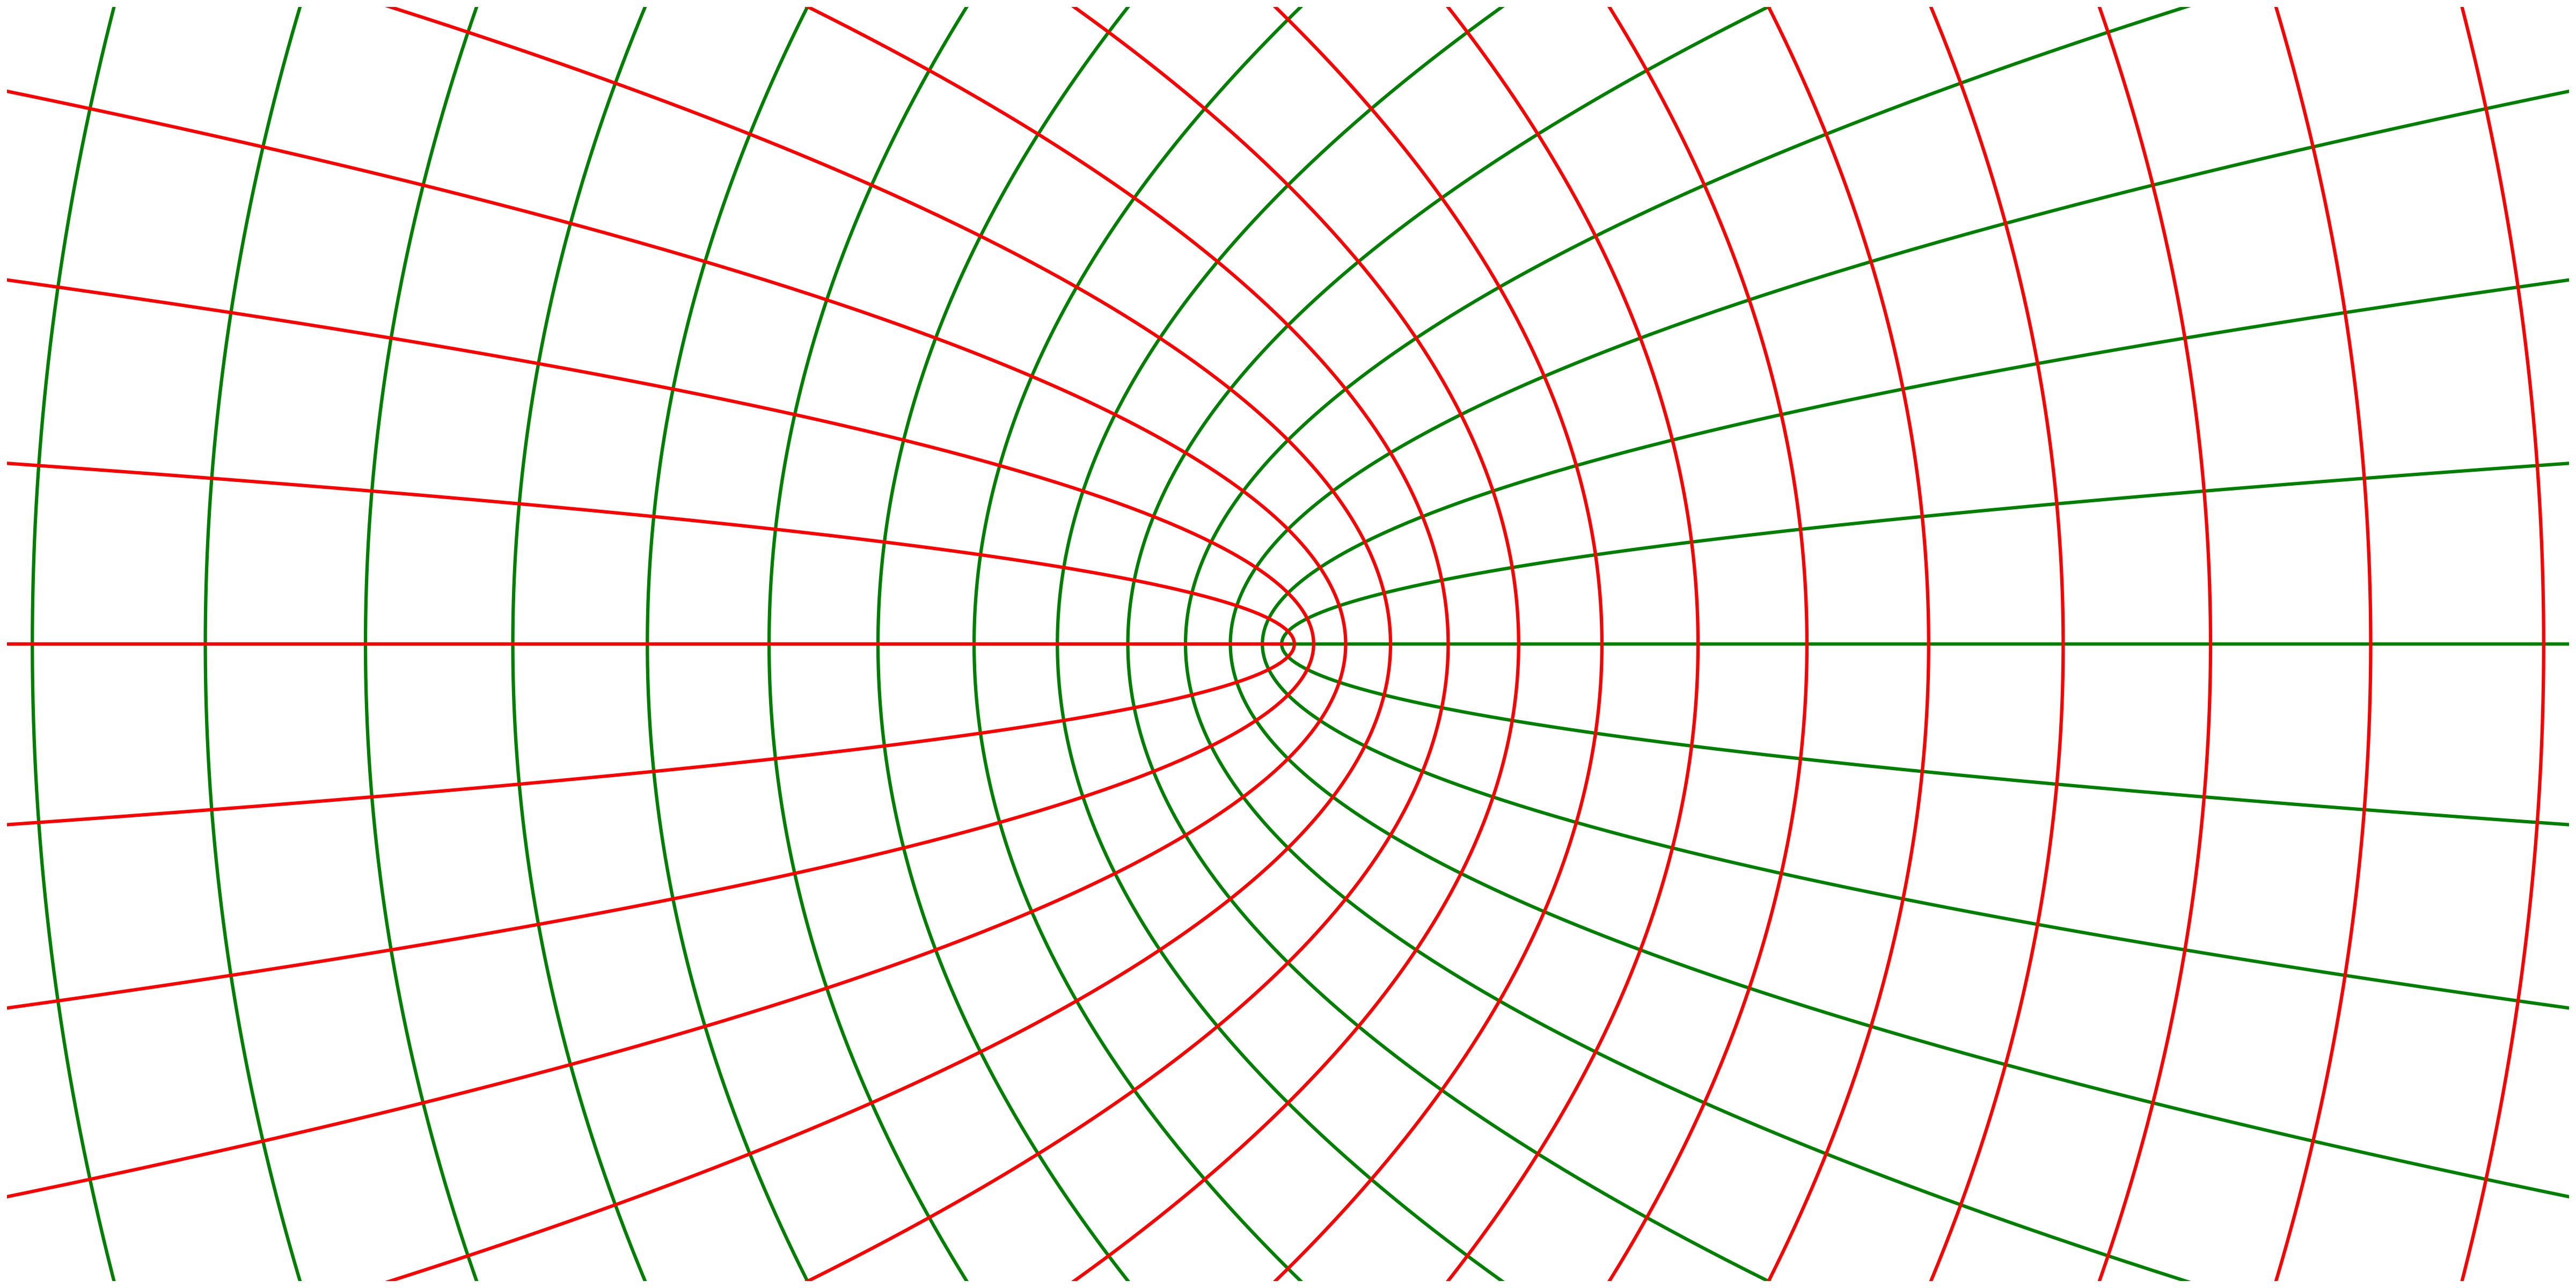
\includegraphics[scale=0.32]{papers/parzyl/img/coordinates.png}
    \caption{Das parabolische Koordinatensystem. Die grünen Parabeln haben ein 
    konstantes $\sigma$ und die roten ein konstantes $\tau$.}
    \label{parzyl:fig:cordinates}
\end{figure}
Abbildung \ref{parzyl:fig:cordinates} zeigt das parabolische Koordinatensystem.
Das parabolische Zylinderkoordinatensystem entsteht wenn die Parabeln aus der
Ebene gezogen werden. 
Die Flächen mit $\tau = 0$ oder $\sigma = 0$ stellen somit Halbebenen entlang der $z$-Achse dar.

Um in diesem Koordinatensystem integrieren und differenzieren zu 
können braucht es die Skalierungsfaktoren $h_{\tau}$, $h_{\sigma}$ und $h_{z}$ \cite{parzyl:scalefac}.

Eine infinitesimal kleine Distanz $ds$ zwischen zwei Punkten
kann im kartesischen Koordinatensystem als
\begin{equation}
    \left(ds\right)^2 = \left(dx\right)^2 + \left(dy\right)^2 + 
    \left(dz\right)^2
    \label{parzyl:eq:ds}
\end{equation}
ausgedrückt werden.
Die Skalierungsfaktoren werden in einem orthogonalen Koordinatensystem so bestimmt, dass
\begin{equation}
    \left(ds\right)^2 = \left(h_{\sigma}d\sigma\right)^2 + 
    \left(h_{\tau}d\tau\right)^2 + \left(h_z dz\right)^2
\label{parzyl:eq:dspara}
\end{equation}
gilt.
Dafür werden $dx$, $dy$, und $dz$ in \eqref{parzyl:eq:ds} mit den Beziehungen
von \eqref{parzyl:coordRelationsa} - \eqref{parzyl:coordRelationse} als
\begin{align}
    dx  &= \frac{\partial x }{\partial \sigma} d\sigma + 
        \frac{\partial x }{\partial \tau} d\tau + 
        \frac{\partial x }{\partial \tilde{z}} d \tilde{z} 
        = \tau d\tau - \sigma d \sigma \\
    dy &= \frac{\partial y }{\partial \sigma} d\sigma + 
        \frac{\partial y }{\partial \tau} d\tau +
        \frac{\partial y }{\partial \tilde{z}} d \tilde{z} 
        = \tau d\sigma + \sigma d \tau  \\
    dz &= \frac{\partial \tilde{z} }{\partial \sigma} d\sigma + 
        \frac{\partial \tilde{z} }{\partial \tau} d\tau +
        \frac{\partial \tilde{z} }{\partial \tilde{z}} d \tilde{z} 
        = d \tilde{z}
\end{align}
substituiert.
Wird diese Gleichung in der Form von \eqref{parzyl:eq:dspara}
geschrieben, resultiert
\begin{equation}
    \left(d s\right)^2 = 
        \left(\sigma^2 + \tau^2\right)\left(d\sigma\right)^2 + 
        \left(\sigma^2 + \tau^2\right)\left(d\tau\right)^2 +
        \left(d \tilde{z}\right)^2.
\end{equation}
Daraus ergeben sich die Skalierungsfaktoren 
\begin{align}
    h_{\sigma} &= \sqrt{\sigma^2 + \tau^2}\\
    h_{\tau} &= \sqrt{\sigma^2 + \tau^2}\\
    h_{z} &= 1.
\end{align}
\subsection{Differentialgleichung}
Möchte man eine Differentialgleichung im parabolischen 
Zylinderkoordinatensystem aufstellen, müssen die Skalierungsfaktoren
mitgerechnet werden.
Der Laplace Operator wird dadurch zu
\begin{equation}
    \Delta f = \frac{1}{\sigma^2 + \tau^2} 
        \left( 
            \frac{\partial^2 f}{\partial \sigma ^2} +
            \frac{\partial^2 f}{\partial \tau ^2}
        \right)
        + \frac{\partial^2 f}{\partial z^2}.
    \label{parzyl:eq:laplaceInParZylCor}
\end{equation}
\subsubsection{Lösung der Helmholtz-Gleichung im parabolischen Zylinderfunktion}
Die Differentialgleichungen, welche zu den parabolischen Zylinderfunktionen führen, tauchen
%, wie bereits erwähnt, 
dann auf, wenn die Helmholtz-Gleichung
\begin{equation}
	\Delta f(x,y,z) = \lambda f(x,y,z) 
\end{equation}
im parabolischen Zylinderkoordinatensystem
\begin{equation}
	\Delta f(\sigma,\tau,z) = \lambda f(\sigma,\tau,z) 
\end{equation}
gelöst wird.
%Wobei der Laplace Operator $\Delta$ im parabolischen Zylinderkoordinatensystem gegeben ist als
%\begin{equation}
%	\Delta 
%	= 
%	\frac{1}{\sigma^2 + \tau^2}
%	\left ( 
%	\frac{\partial^2}{\partial \sigma^2} 
%	+ 
%	\frac{\partial^2}{\partial \tau^2}
%	\right )
%	+ 
%	\frac{\partial^2}{\partial z^2}.
%\end{equation}
Mit dem Laplace Operator aus \eqref{parzyl:eq:laplaceInParZylCor} lautet die Helmholtz-Gleichung
\begin{equation}
	\Delta f(\sigma, \tau, z)
	=
	\frac{1}{\sigma^2 + \tau^2}
	\left ( 
	\frac{\partial^2 f(\sigma,\tau,z)}{\partial \sigma^2} 
	+ 
	\frac{\partial^2 f(\sigma,\tau,z)}{\partial \tau^2}
	\right )
	+ 
	\frac{\partial^2 f(\sigma,\tau,z)}{\partial z^2}
	= 
	\lambda f(\sigma,\tau,z).
\end{equation}
Diese partielle Differentialgleichung kann mit Hilfe von Separation gelöst werden, dazu wird 
\begin{equation}
	f(\sigma,\tau,z) = g(\sigma)h(\tau)i(z)
\end{equation}
gesetzt, was dann schlussendlich zu den Differentialgleichungen 
\begin{equation}\label{parzyl:sep_dgl_1}
	g''(\sigma) 
	- 
	\left (
	\lambda\sigma^2
	+
	\mu 
	\right )
	g(\sigma)
	=
	0,
\end{equation}
\begin{equation}\label{parzyl:sep_dgl_2}
	h''(\tau) 
	- 
	\left (
	\lambda\tau^2
	-
	\mu 
	\right )
	h(\tau)
	=
	0
\end{equation}
und
\begin{equation}\label{parzyl:sep_dgl_3}
	i''(z) 
	+
	\left (
	\lambda
	+
	\mu 
	\right )
	i(z)
	=
	0
\end{equation}
führt. $\lambda$ und $\mu$ sind dabei die Separationskonstanten. 
\eqref{parzyl:sep_dgl_1} und \eqref{parzyl:sep_dgl_2} sind auch 
als Webersche Differentialgleichungen bekannt.



